\section{Documentation and Metadata}

Data documentation and the generation of metadata is essential to understand
your data in detail, and also help other researchers find, use and properly
cite your data.


Various and particular metadata standards are available for each discipline, and
you have to find them by yourself. Further general guidelines are provided below.

\subsection{Important things to do while you collect or create your data}

\begin{itemize}
  \item Make a note of all file names and formats associated with the project,
        how the data is organized, how the data was generated (including any
        equipment or software used), and information about how the data has been
        altered or processed.
  \item Include an explanation of codes, abbreviations, or variables used in the
        data or in the file naming structure.
  \item Keep notes about where you got the data so that you and others
        can find it.
\end{itemize}

\subsection{Things to document about your data}\label{sc:data-documentation}

The used metadata scheme follows the recommendation of the world wide DataCite
consortium (TIB Hannover, Britisch Library, Denmark Technical Information
Center, ETH Zurich, CalTech, Australian National Data Service, ...). These data
are stored in a “readme.json” file in \textbf{\underline{EVERY DIRECTORY}} of
your data! Please, use our ‘Readme File Creator’ described below to generate
this file. \\
\begin{wrapfigure}{r}{0.5\linewidth}
  \vspace{-1em}
  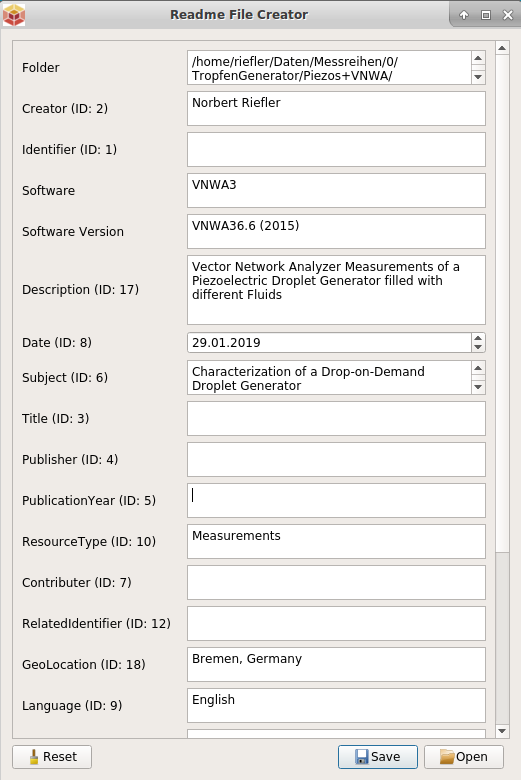
\includegraphics[width=\linewidth]{Figure02_ReadmeFileCreator.png}
  \caption{Data Input Tool: Readme-File-Creator}
  \label{fig:readme-creator}
\end{wrapfigure}
Explanation of some extracted properties are given in the following; please
refer to Table 3 in \cite{datacite2019} for more information: \\[6pt]
%
\textbf{ID 1: Identifier} \\
Number used to identify the data. Can be a DOI (Digital Object Identifier) in
case of a paper, or an ID from the ELN (eLabFTW generates a long number for
every experiment, see below) \\[6pt]
%
\textbf{ID 2: Creator} \\
Name of the person responsible for the described data (ORCID). \\[6pt]
%
\textbf{ID 3: Title}
May be the title of a dataset, or the name of a piece of software, or the
title of a paper. \\[6pt]
%
\textbf{ID 4: Publisher} \\
The name of the entity that produces, holds, archives, publishes prints,
distributes, releases or issues the resource (e.g. “Leibniz Institute for
Materials Engineering IWT”). \\[6pt]

\pagebreak
\noindent\textbf{ID 5: Publication Year} \\
The year when the data was or will be made publicly available. \\[6pt]
%
\textbf{ID 8: Date} \\
Key date associated with the data, e.g. project start, end date, data
modification, data release date, or time period covered by the data \\[6pt]
%
\textbf{ID 9: Language} \\
Language(s) of the intellectual content of the resource, when applicable \\[6pt]
%
\textbf{ID 10: Resource Type} \\
A description of the resource; mostly ‘DataSet’, but may be ‘Audiovisual’,
‘High-Speed Images’, ‘DataPaper’, etc. \\[6pt]
%
\textbf{ID 19: Funding Reference} \\
Organizations or agencies who funded the research \\[6pt]
%
\textbf{ID 16: Rights} \\
Any known intellectual property rights held for the data. The best choice is
either the Creative Commons license 'CC-BY' (BY attribution) or 'CC-0' for
data and 'CC Version 4.0' for written documents. \\[6pt]
%
\textbf{ID 17: Description} \\
How the data was generated, including equipment or software used, experimental
protocol, other things you might include in a lab notebook \\[6pt]
%
\textbf{ID 18: Geolocation} \\
When the data relates to a physical location, record information about its
spatial coverage \\[6pt]
%
This tool displayed in figure \ref{fig:readme-creator} can be downloaded
from the VT-Server \\ (/VT-Allgemein/Software/ReadmeFile-Creator) for every
operating system to simplify metadata entry (figure on the right). You can
create automatically a file called ‘readme.json’ with your metadata, embedded
in a JSON (Java Scipt Object Notation) format, which is used as documentation as
well as metadata for Data Science Methods. This file is stored in every
directory which contains data or program code.\\
%
The same DataCite metadata structure can be included into the ELN (see \ref{ssc:ELN}).
